\chapter{Use case}

%begin free user section
\section{Free-user}
	\subsection{General Use Case}
		\begin{figure}[ht]
			\begin{center}
				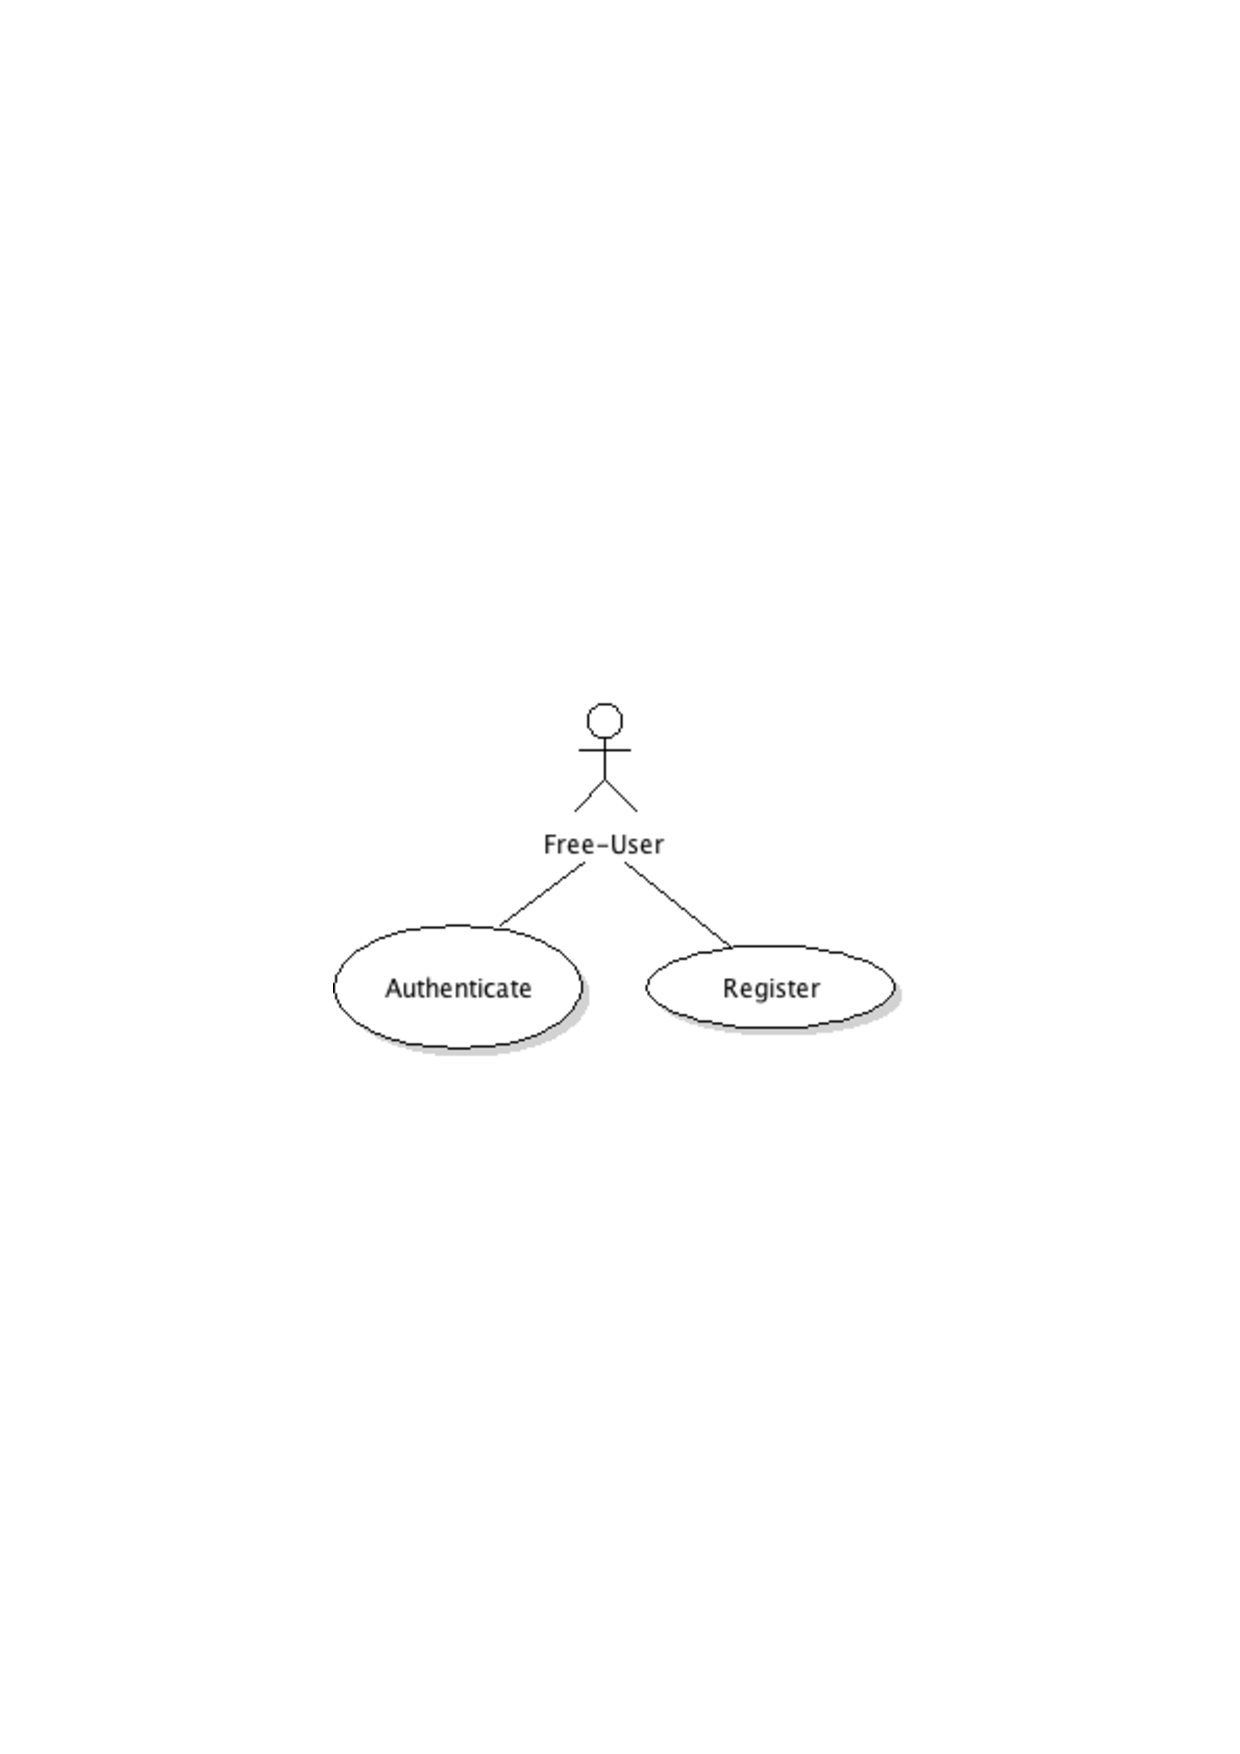
\includegraphics[width=\textwidth,  trim=2cm 10cm 2cm 11cm]{UML_figure/UC/free_user/UC_FreeUser_General.pdf}
				\caption{Free-User Use Case : Overview}
			\end{center}
		\end{figure}
		A free user is a user non identified by the platform. He has the following features~:
	\subsection{Register}Register a free-user to have access to the different features.
	\subsection{Authenticate}Identify free-user and if registered give him access to the different features.
%end free user section
\newpage
%begin student section
\section{Student}
	\subsection{General Use Case}
		\begin{figure}[ht]
			\begin{center}
				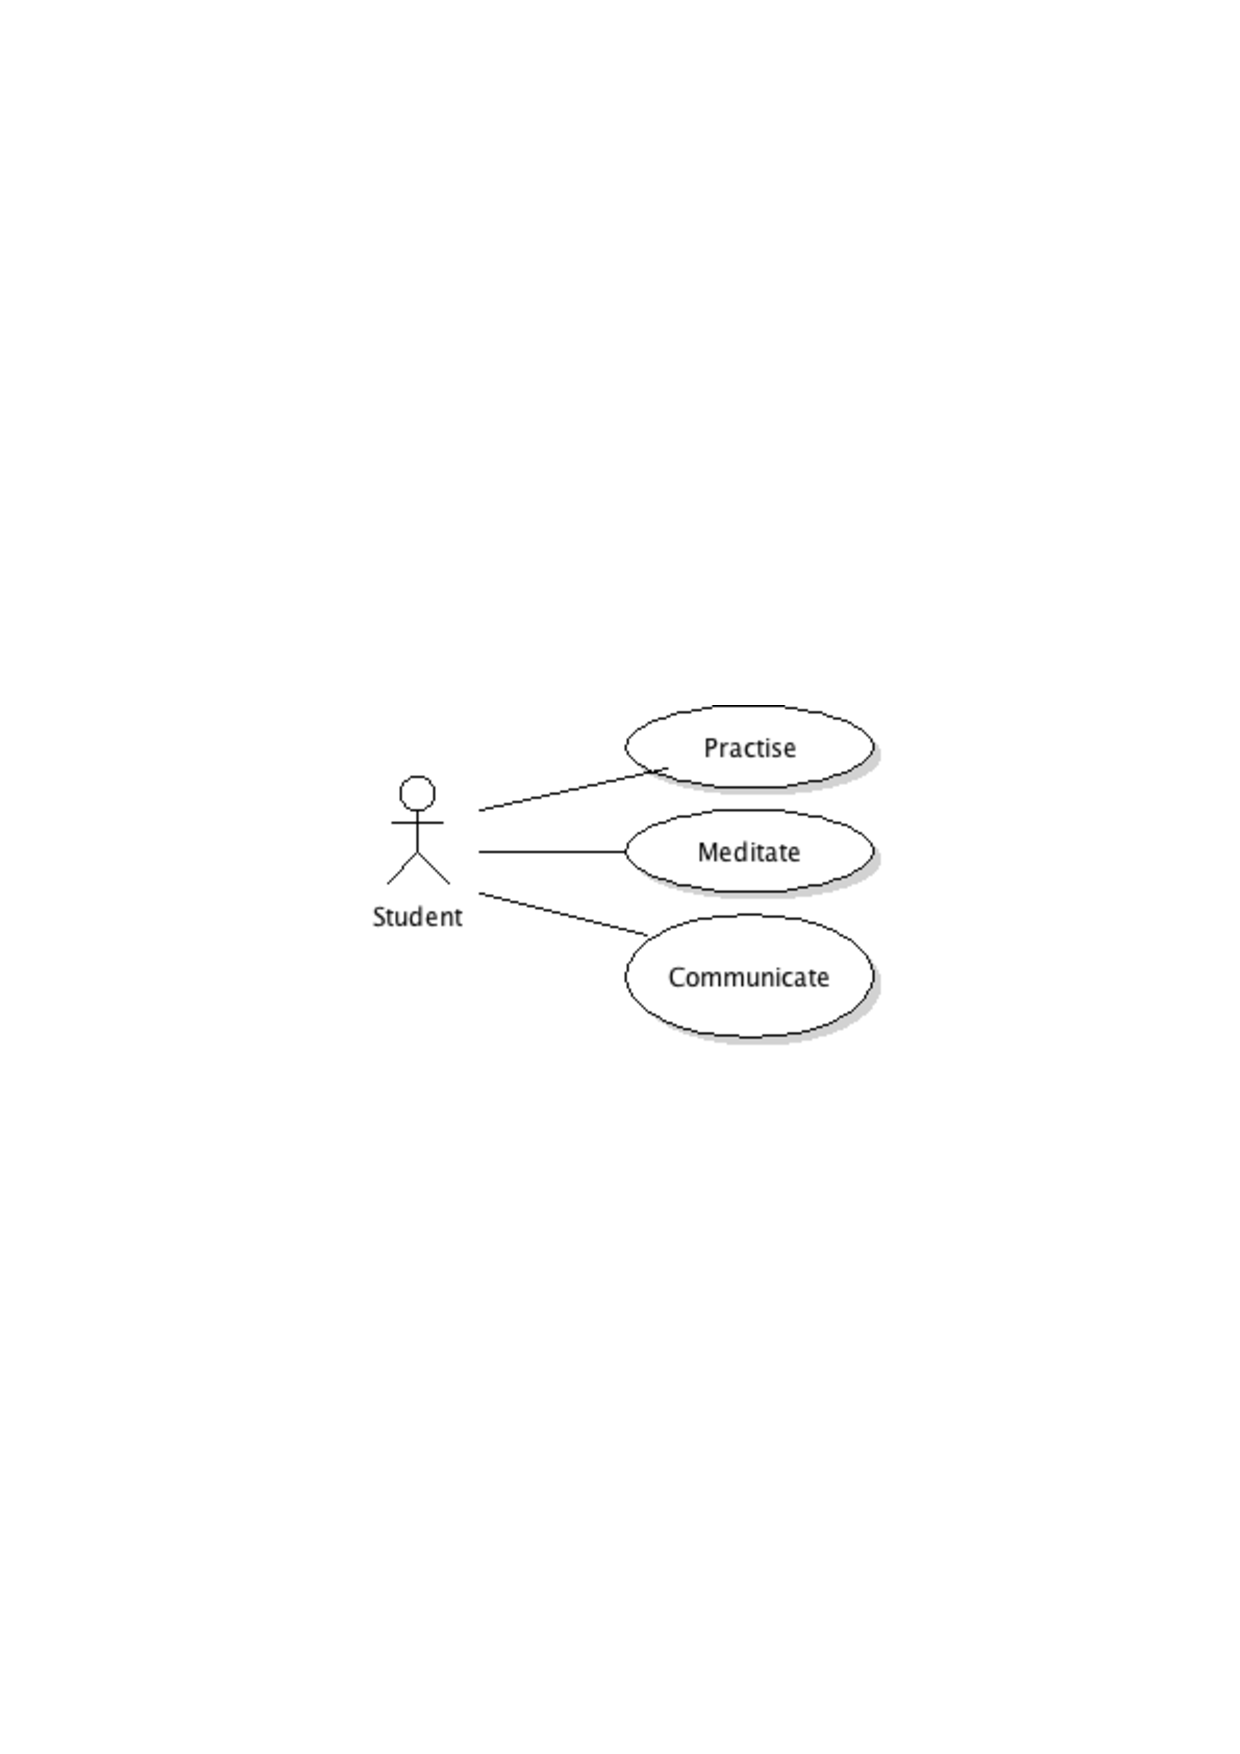
\includegraphics[width=\textwidth,  trim=2cm 10cm 2cm 11cm]{UML_figure/UC/student/UC_Student_General.pdf}
				\caption{Student Use Case : Overview}
			\end{center}
		\end{figure}
		A user identify as a student has three major action which are Practise, Meditate and Communicate.
	\subsection{Practise}
		\begin{figure}[ht]
			\begin{center}
				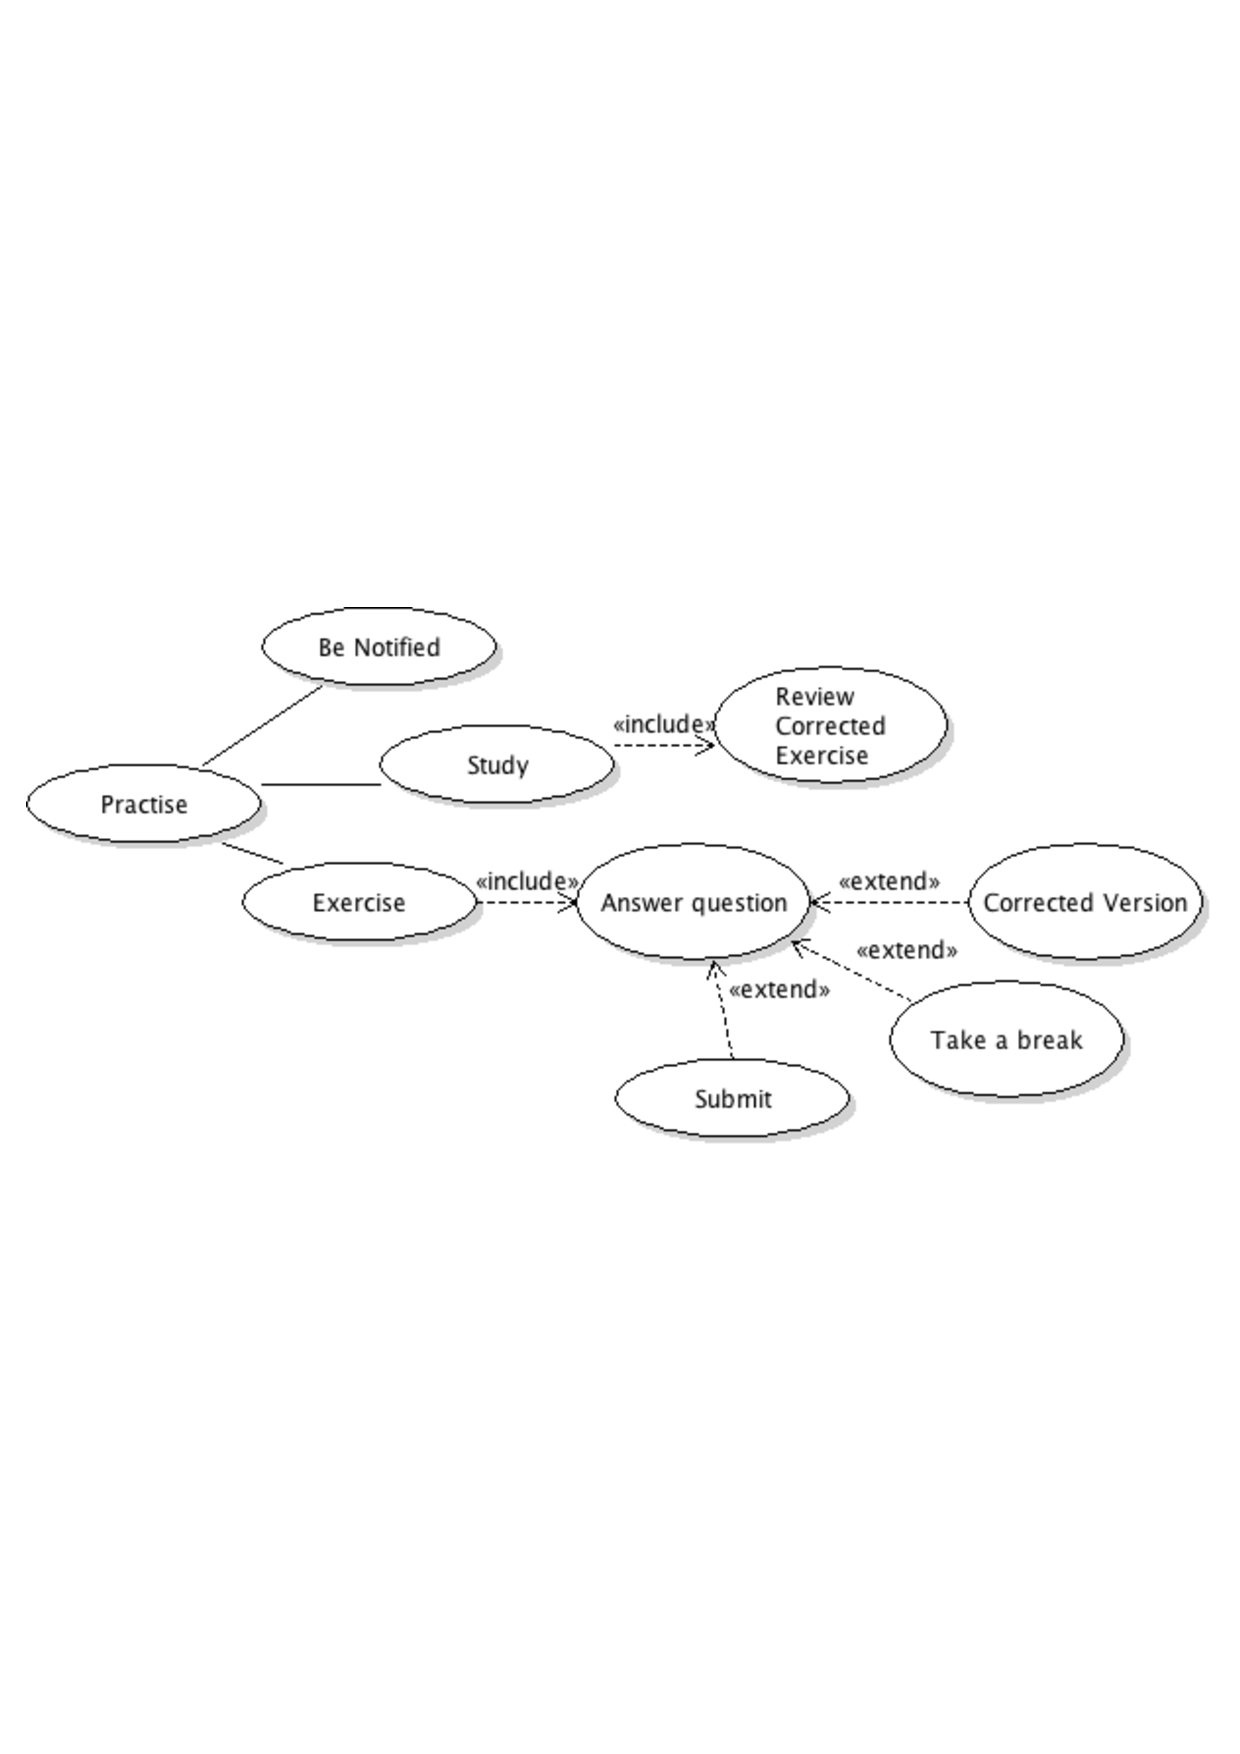
\includegraphics[width=\textwidth,  trim=2cm 10cm 2cm 11cm]{UML_figure/UC/student/UC_Student_Practise.pdf}
				\caption{Student Use Case : Practise}
			\end{center}
		\end{figure}
		\subsubsection{Be notified}
			The student will be notified when he/she has new exercises to do, or to finish.
		\subsubsection{Exercise}
			The student can exercises himself by doing exercises written by the teacher.
		\subsubsection{Answer Question}
			The student will answer question such as MCQ (Multiple Choice Question)
		\subsubsection{Take a break}
			He/she can take a break and resume the exercise later.
		\subsubsection{Corrected Version}
			A corrected version of the question will be available if the teacher has checked the option.
		\subsubsection{Study}
			The student can study by reviewing corrected exercises.
	\subsection{Meditate}
		\begin{figure}[ht]
			\begin{center}
				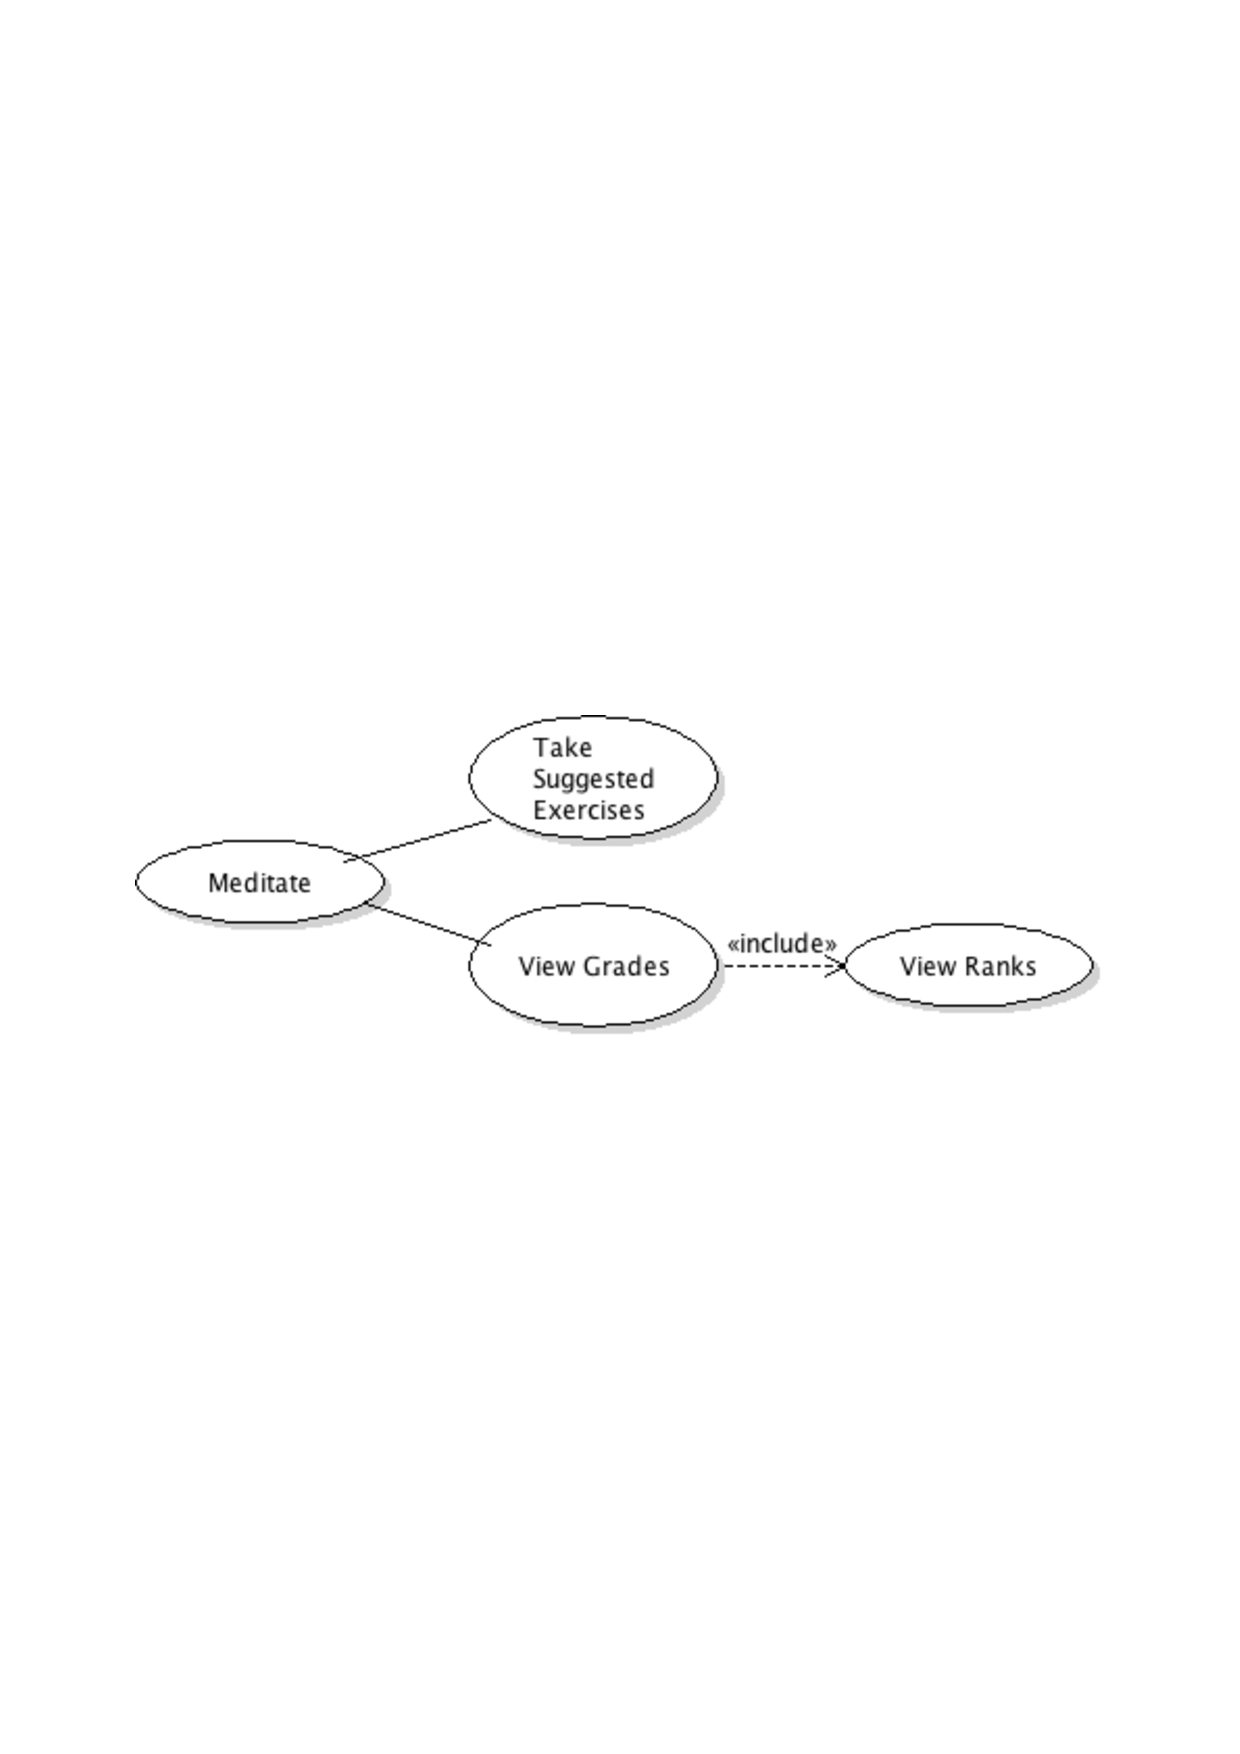
\includegraphics[width=\textwidth,  trim=2cm 10cm 2cm 11cm]{UML_figure/UC/student/UC_Student_Meditate.pdf}
				\caption{Student Use Case : Meditate}
			\end{center}
		\end{figure}
		\subsubsection{Suggested Exercises}
			The platform will provide exercises according to the student grade on each exercises.
		\subsubsection{Grade}
			Student can see their grade for each exercises.
		\subsubsection{Rank}
			Student can compare himself with other student.
%end student section
\newpage
%begin teacher section
\section{Teacher}
	\subsection{General Use Case}
		\begin{figure}[ht]
			\begin{center}
				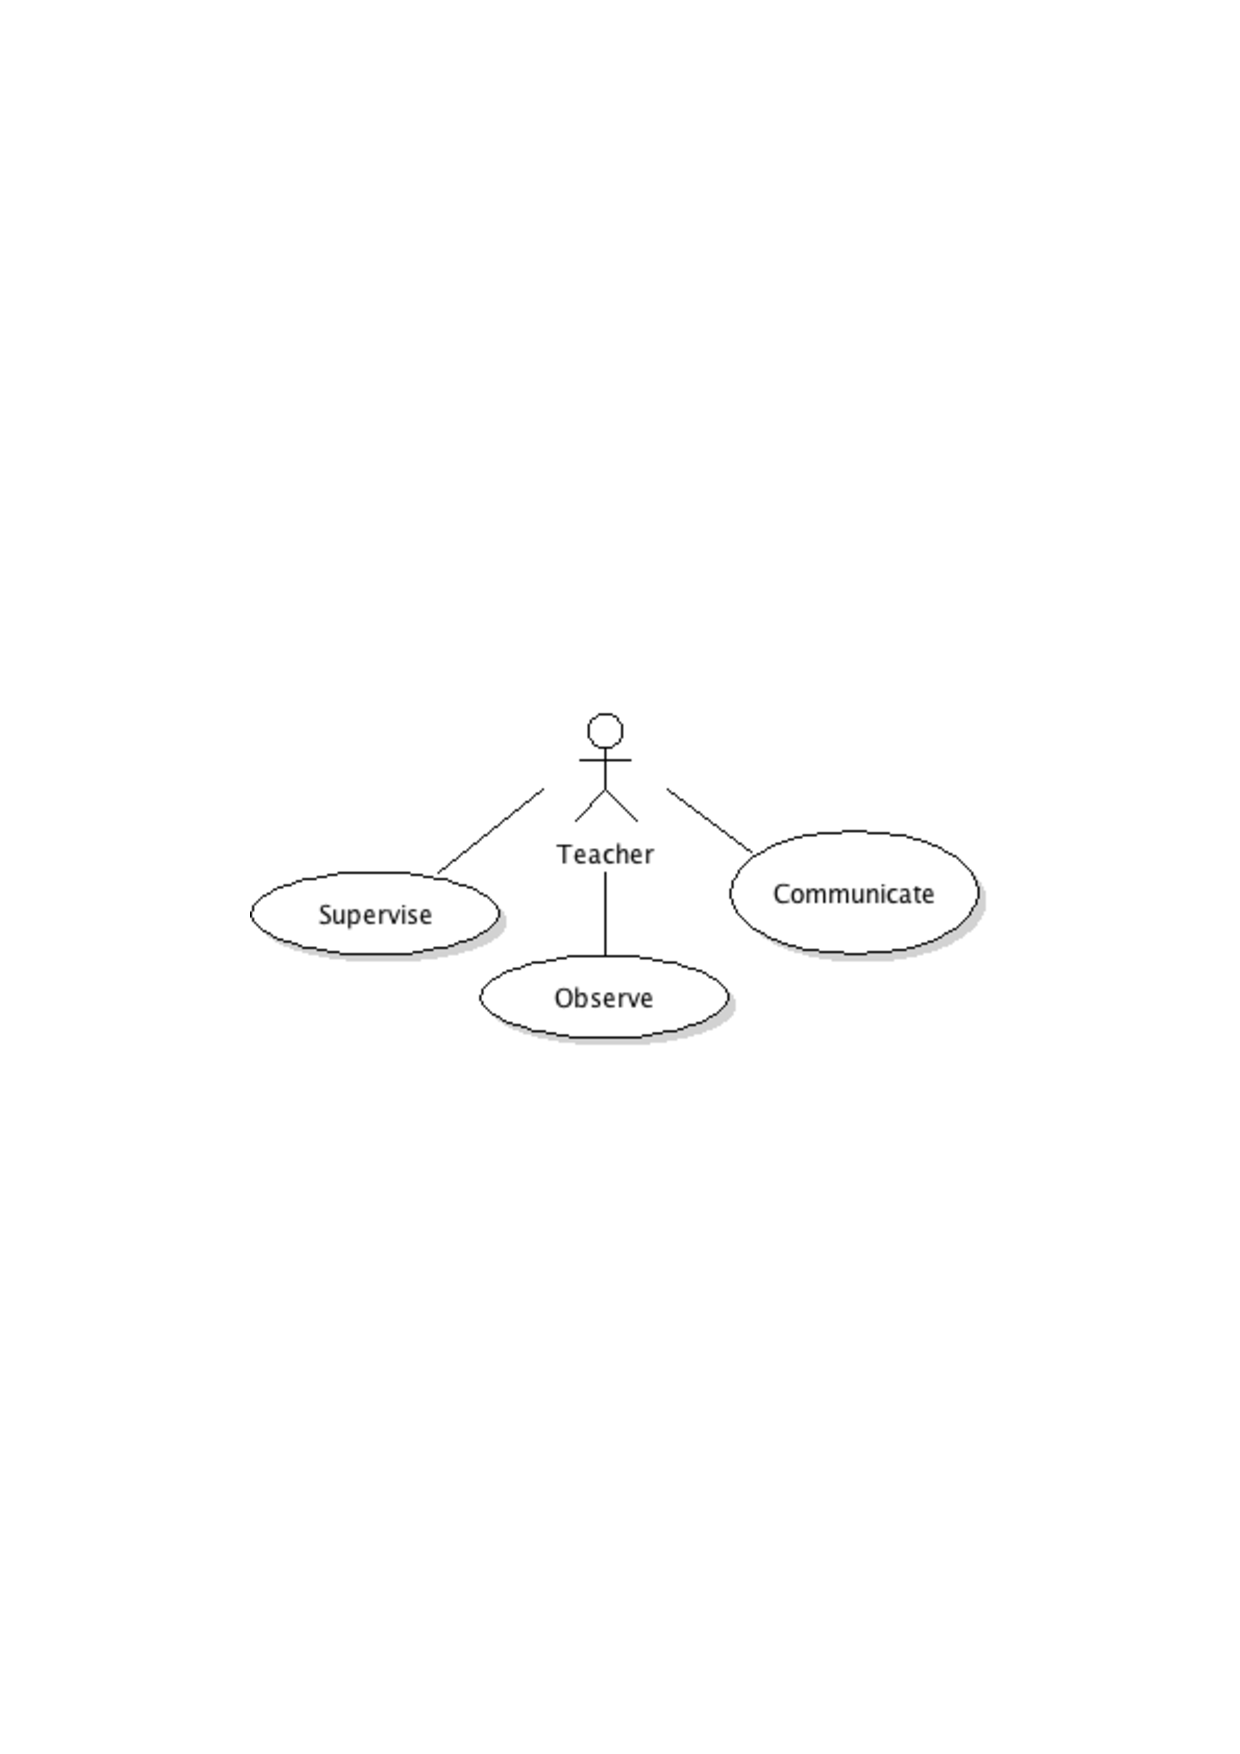
\includegraphics[width=\textwidth,  trim=2cm 10cm 2cm 11cm]{UML_figure/UC/teacher/UC_Teacher_General.pdf}
				\caption{Teacher Use Case : Overview}
			\end{center}
		\end{figure}
		Main Features for the teacher are Supervise, Observe, Communicate
	\subsection{Supervise}
		\begin{figure}[ht]
			\begin{center}
				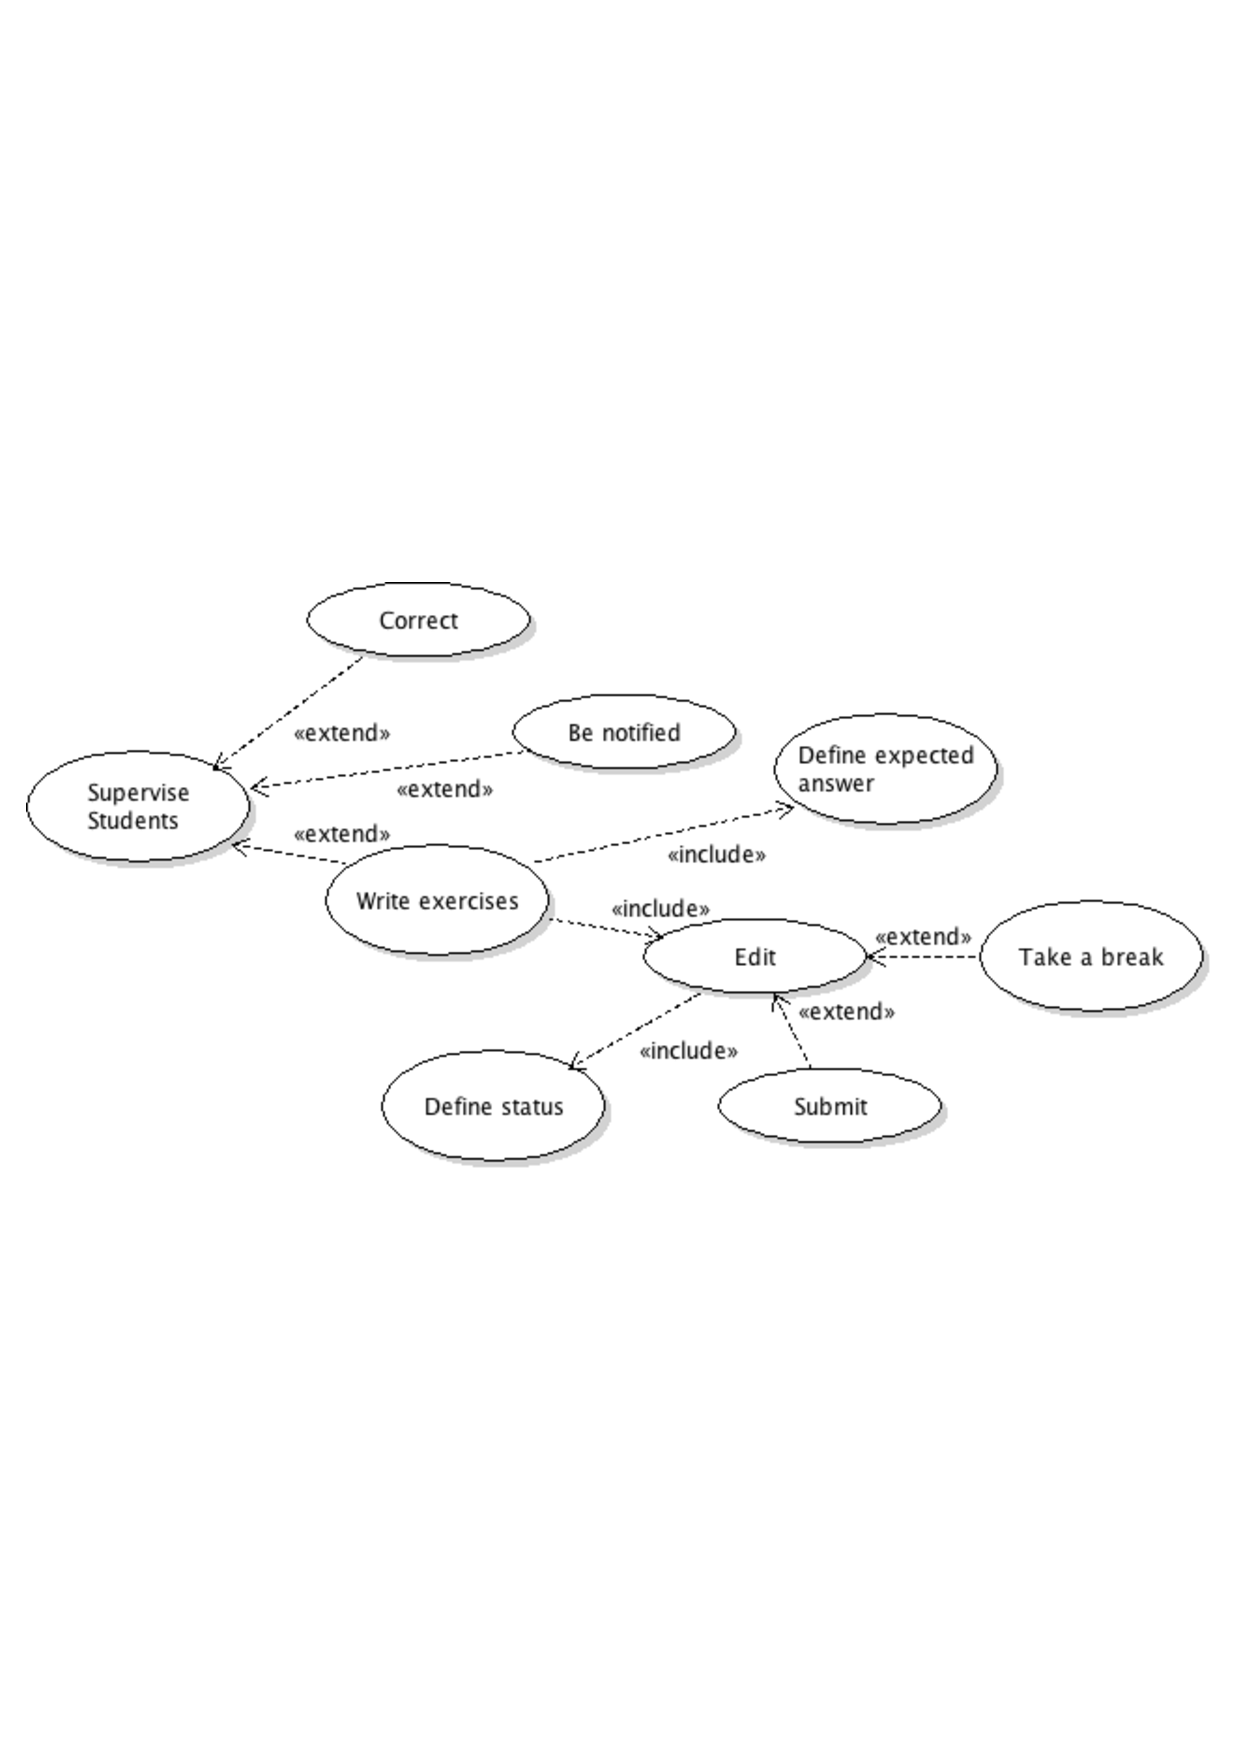
\includegraphics[width=\textwidth,  trim=2cm 10cm 2cm 9cm]{UML_figure/UC/teacher/UC_Teacher_Supervise.pdf}
				\caption{Teacher Use Case : Supervise}
			\end{center}
		\end{figure}
		\subsubsection{Be Notified}
			The teacher will be notified when his exercises are online.\\
			He also is notified when he has manual correction to do.
		\subsubsection{Write exercises}
			The teacher supervises his students by writing exercises.
		\subsubsection{Write Corrected Version}
			When a teacher writes exercises he needs to write a corrected version for automatic correction.
		\subsubsection{Edit}
			The exercise he writes can be edited at anytime.
		\subsubsection{Define Status}
			The exercise will have status, teacher have to define status such as date, deadline, priority.\\
			Release condition can also be defined. For instance, every student who fail the exercise 1.4 will be notified this exercise. 
		\subsubsection{Take a break}
			Teacher can take a break about writing his exercise, to resume it later.
		\subsubsection{Submit}
			The teacher submit his exercise which can be viewed by student according to status definition by the teacher.
		\subsubsection{Correct}
			The teacher has to correct questions on which he has not define an answer.
	\newpage
	\subsection{Observe}
		\begin{figure}[ht]
			\begin{center}
				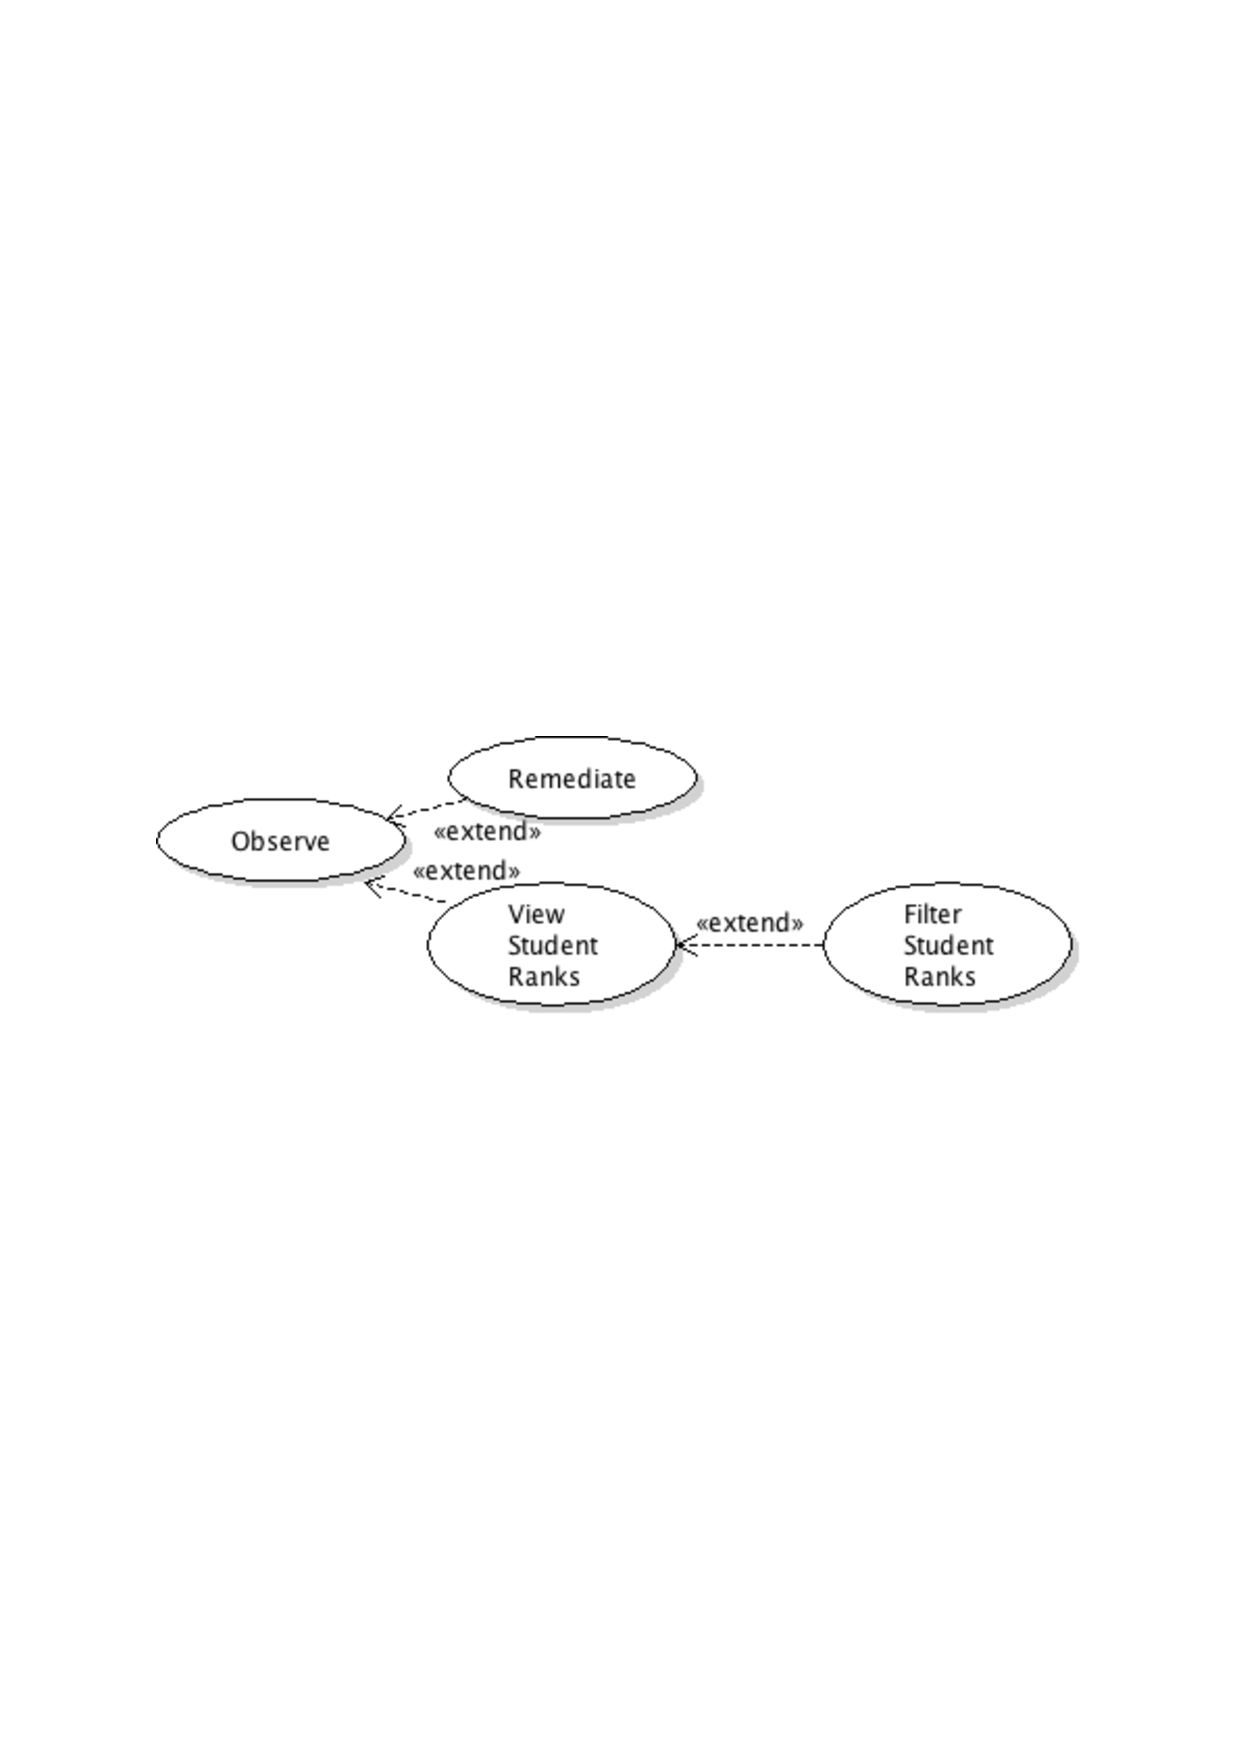
\includegraphics[width=\textwidth,  trim=2cm 10cm 2cm 11cm]{UML_figure/UC/teacher/UC_Teacher_Observe.pdf}
				\caption{Teacher Use Case : Observe}
			\end{center}
		\end{figure}
		\subsubsection{Rank}
			The teacher can see all the grade of students who took his exercises.
		\subsubsection{Filter}
			He can filter the grade according to the group, rising order, the one who have more or less than a mark.
		\subsubsection{Remediate}
			Then the teacher can provide exercises for a group of students in difficulties according to their grade.
%end teacher section
\newpage
%begin administrator section
\section{Administrator}
	\subsection{General Use Case}
		\begin{figure}[ht]
			\begin{center}
				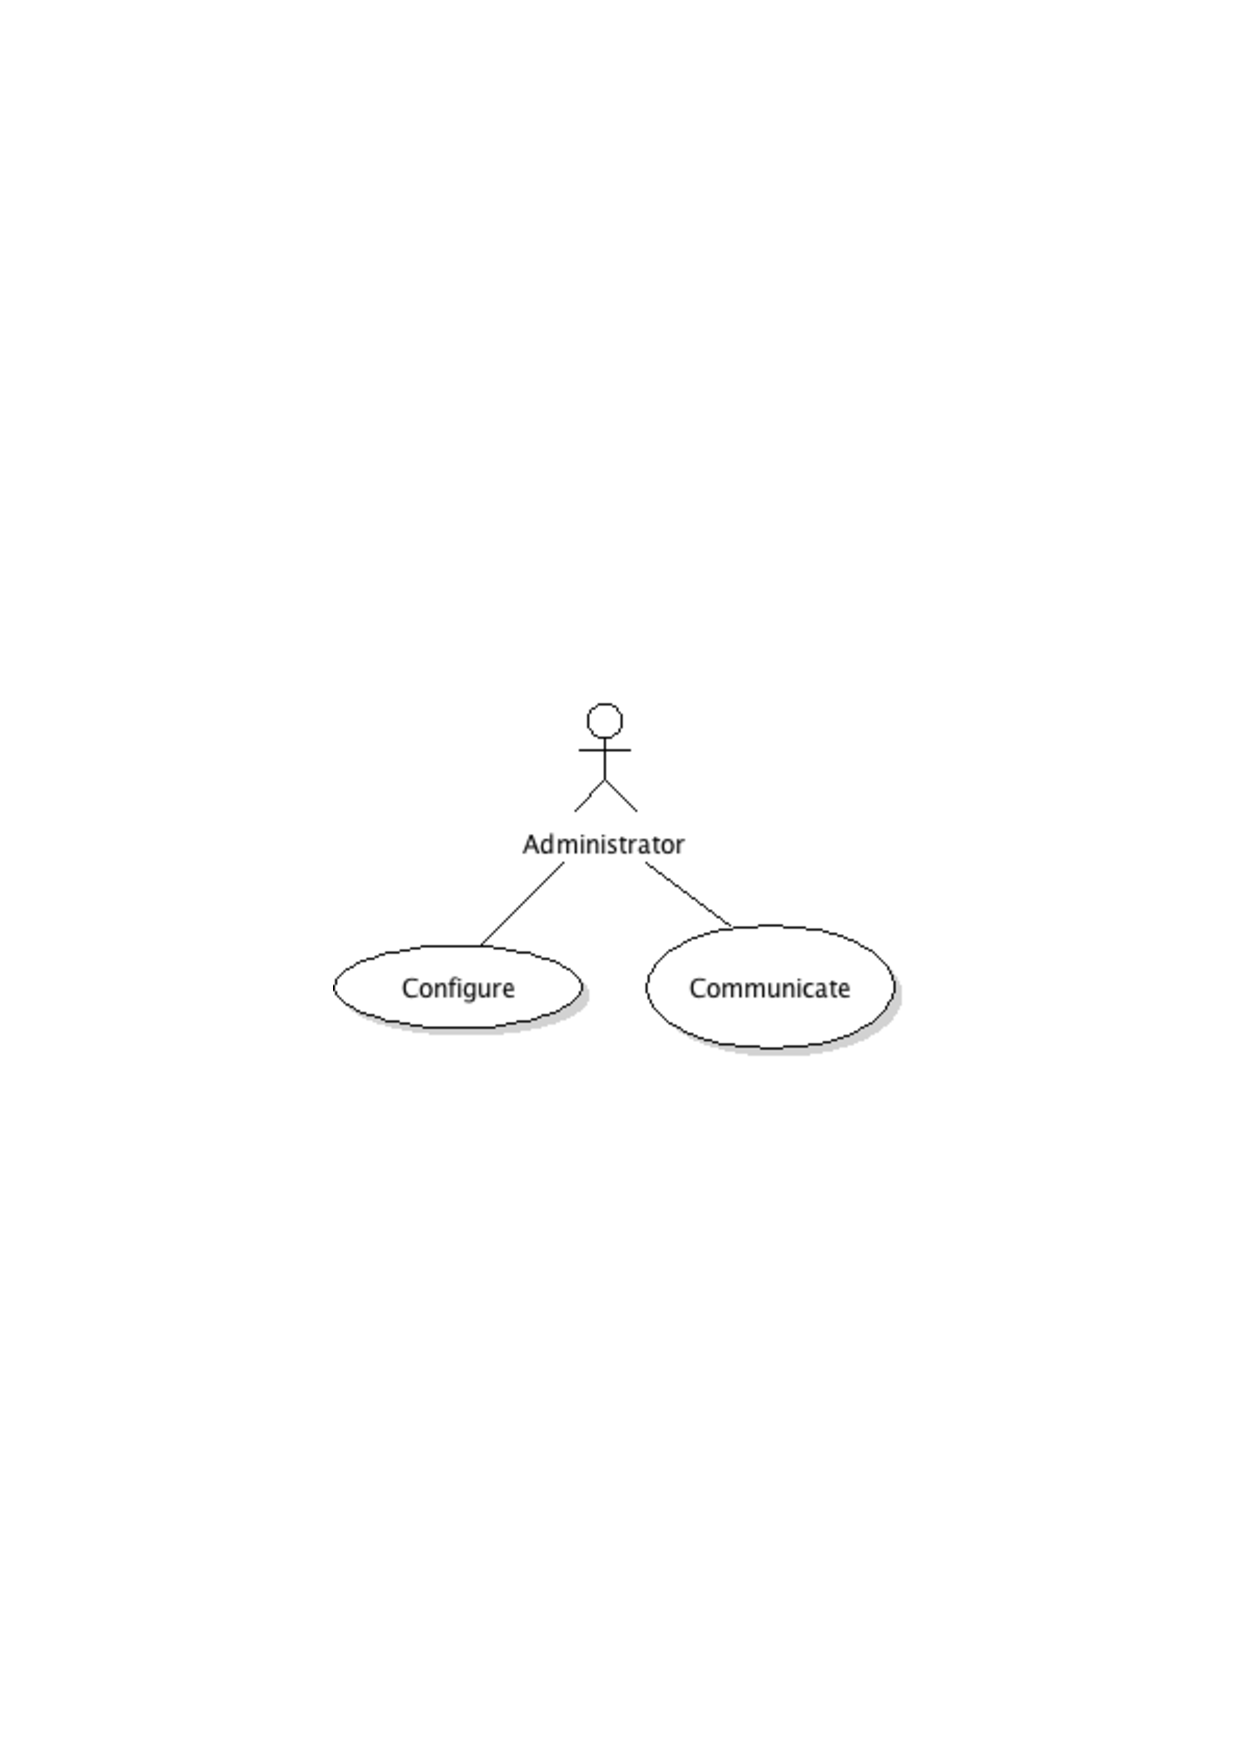
\includegraphics[width=\textwidth, trim=2cm 10cm 2cm 11cm]{UML_figure/UC/administrator/UC_Administrator_General.pdf}
				\caption{Administrator Use Case : Overview}
			\end{center}
		\end{figure}
	\subsection{Configure}
		The administrator task is to configure the platform.
%end administrator section
\newpage
%begin common user section
\section{Common registered user}
	\begin{figure}[ht]
		\begin{center}
			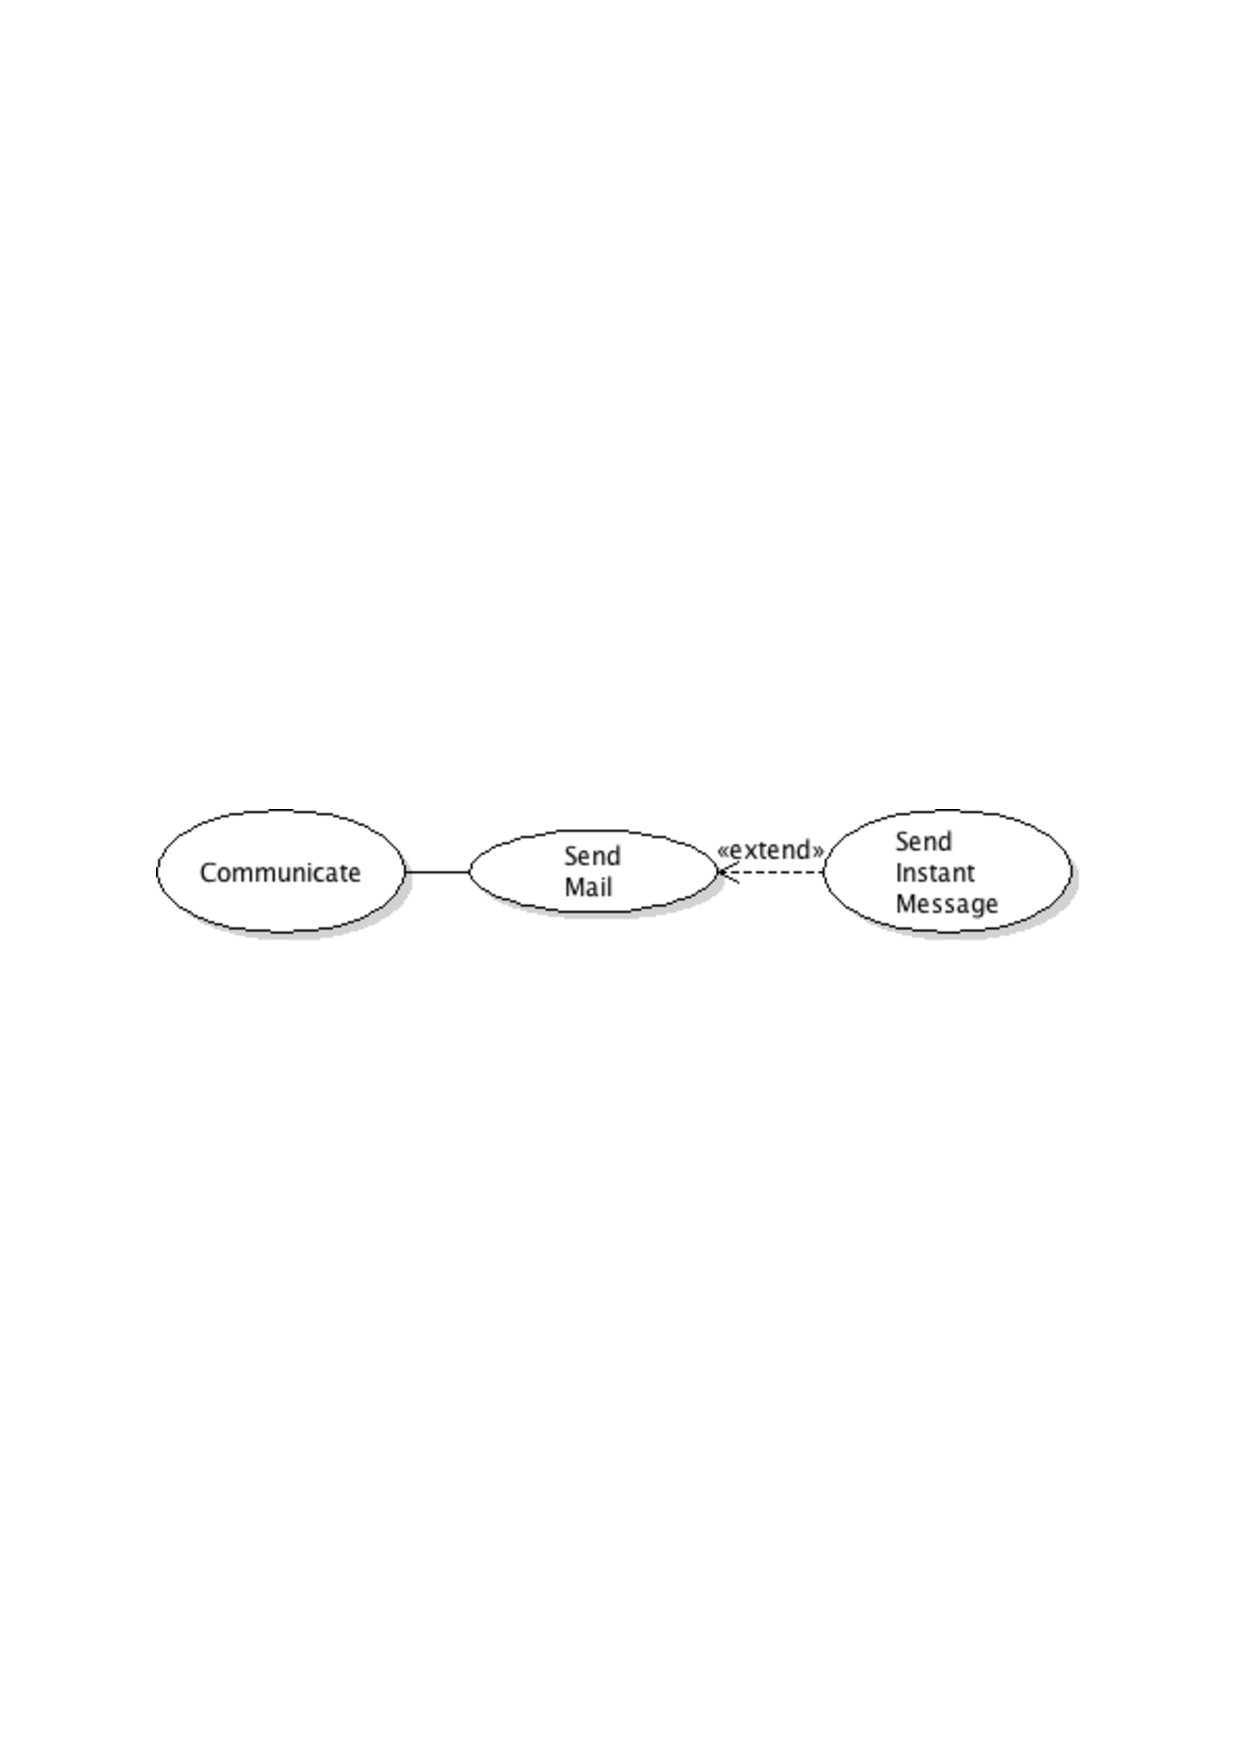
\includegraphics[width=\textwidth,  trim=2cm 10cm 2cm 11cm]{UML_figure/UC/common/UC_Common_Communicate.pdf}
			\caption{Registered user Use Case : Communicate}
		\end{center}
	\end{figure}
	\subsection{Communicate}
		Registered user can communicate each other.
		\subsubsection{Send Mail}
			Communication provide by mail exchange.
		\subsubsection{Send Instant Message}
			Communication provide by instant message exchange.
%end common user section













